\subsection{Beam Line Chambers} \label{sec:BLC}
\begin{figure}[htbp]
  \centering
  \begin{tabular}{ccc}
    \begin{minipage}{0.33\hsize}
      \includegraphics[width=4cm]{../pic/Run78/BL/BLC1_time.eps}
    \end{minipage}
    \begin{minipage}{0.33\hsize}
      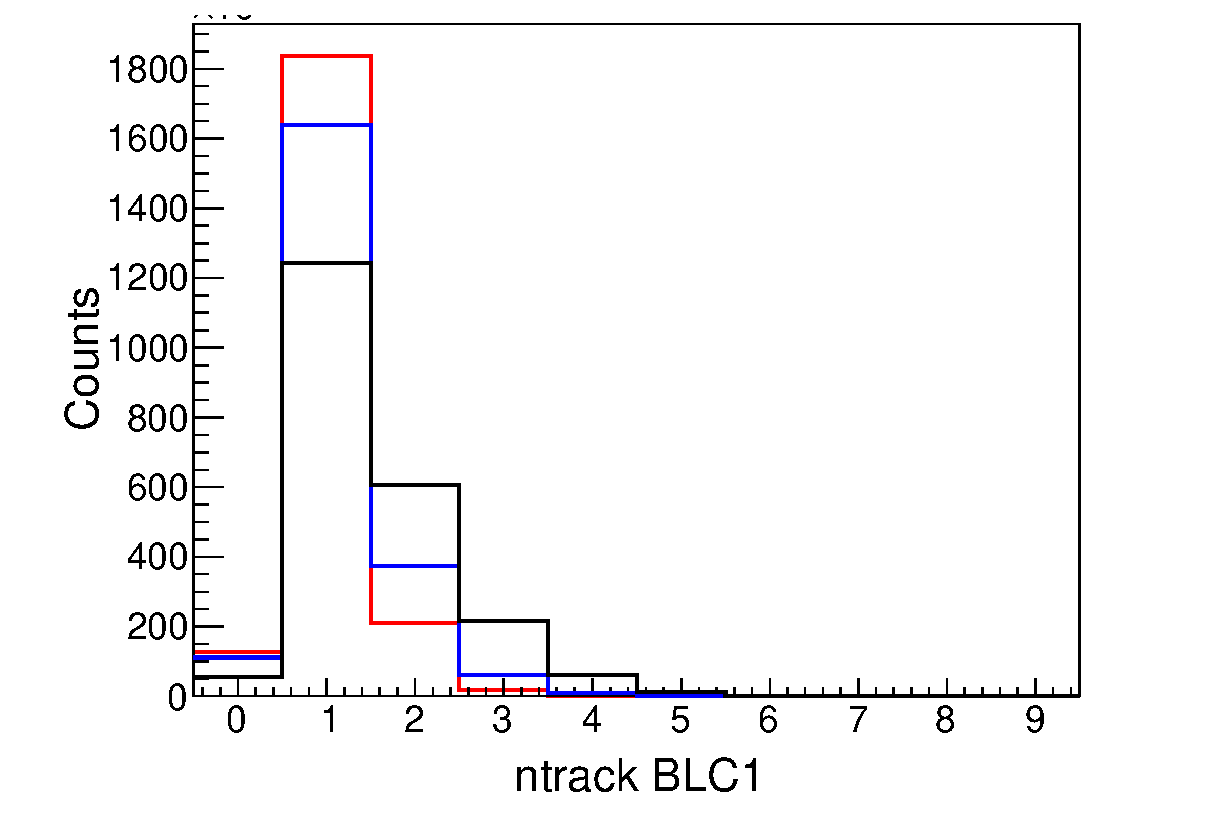
\includegraphics[width=4cm]{../pic/Run78/BL/nBLC1.eps}
    \end{minipage}
    \begin{minipage}{0.33\hsize}
      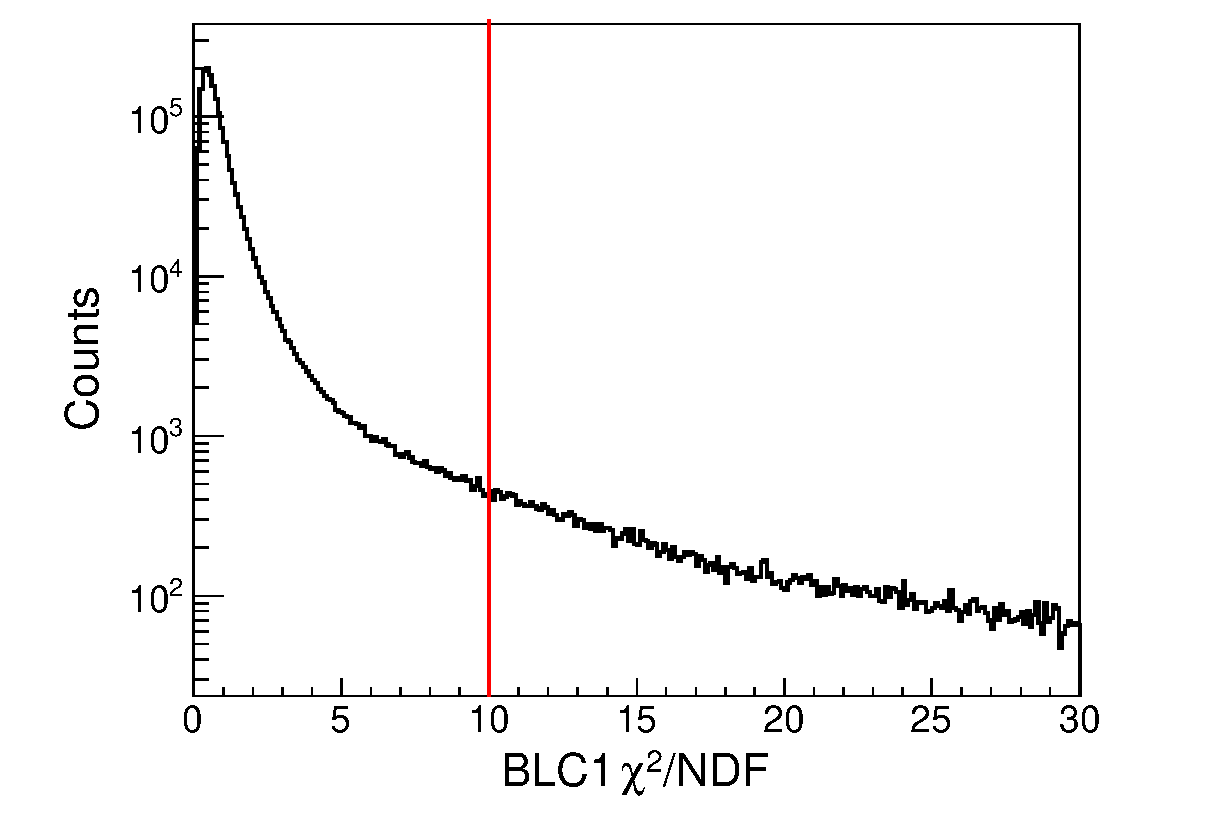
\includegraphics[width=4cm]{../pic/Run78/BL/BLC1_chi2.eps}
    \end{minipage}
  \end{tabular}

  \begin{tabular}{ccc}
    \begin{minipage}{0.33\hsize}
      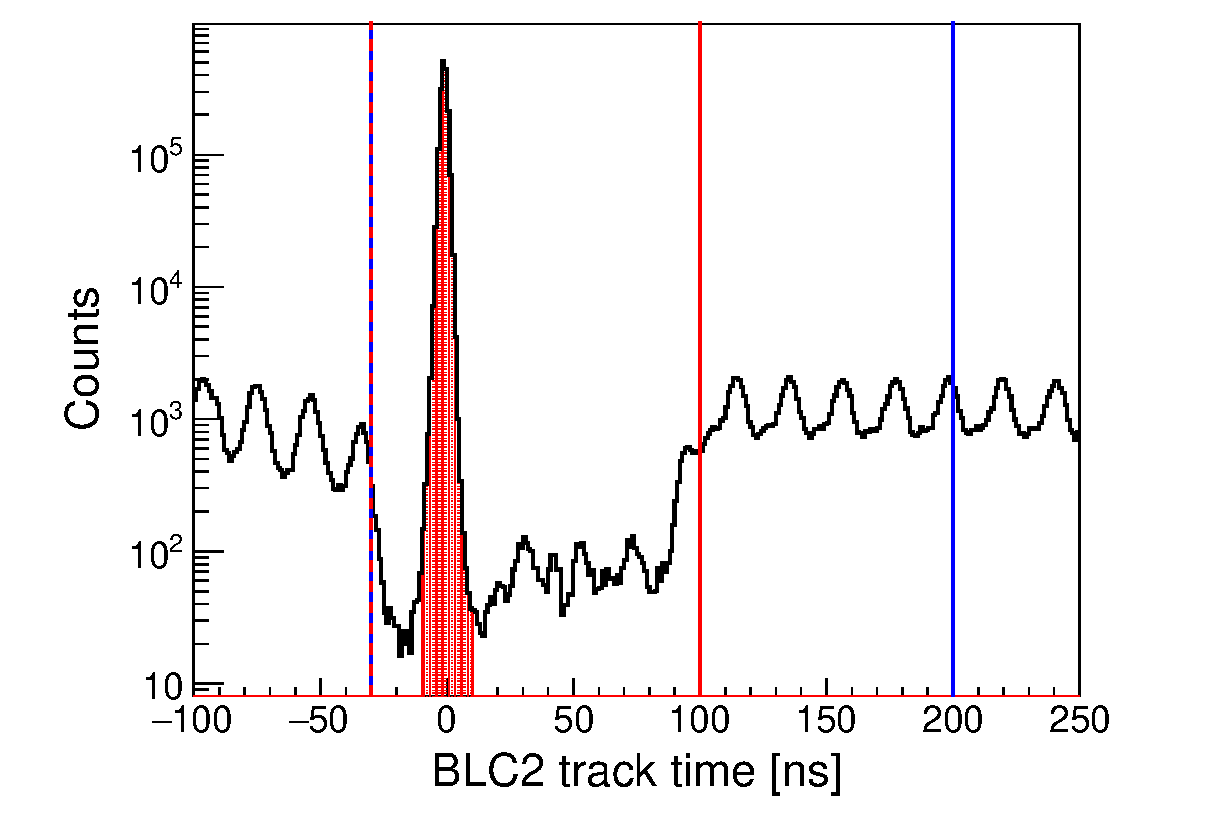
\includegraphics[width=4cm]{../pic/Run78/BL/BLC2_time.eps}
    \end{minipage}
    \begin{minipage}{0.33\hsize}
      \includegraphics[width=4cm]{../pic/Run78/BL/nBLC2.eps}
    \end{minipage}
    \begin{minipage}{0.33\hsize}
      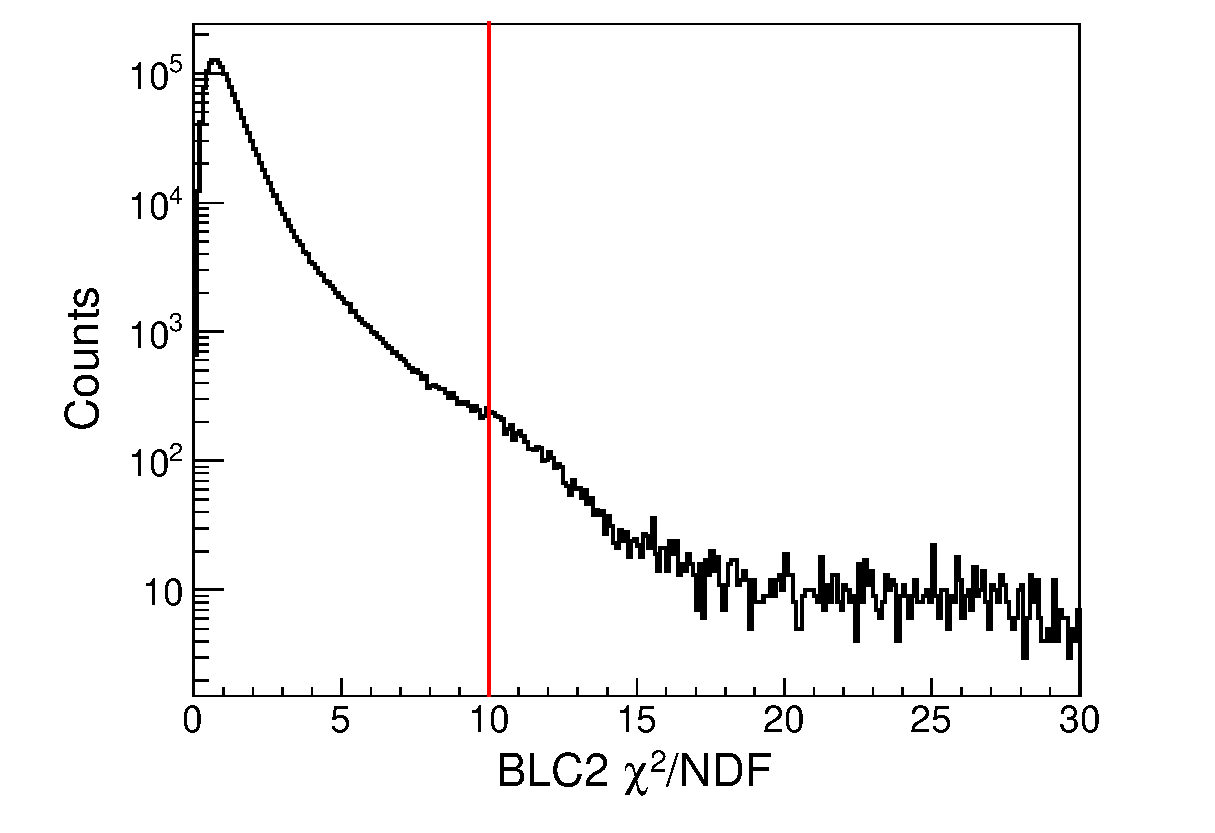
\includegraphics[width=4cm]{../pic/Run78/BL/BLC2_chi2.eps}
    \end{minipage}
  \end{tabular}

    \begin{tabular}{ccc}
    \begin{minipage}{0.33\hsize}
      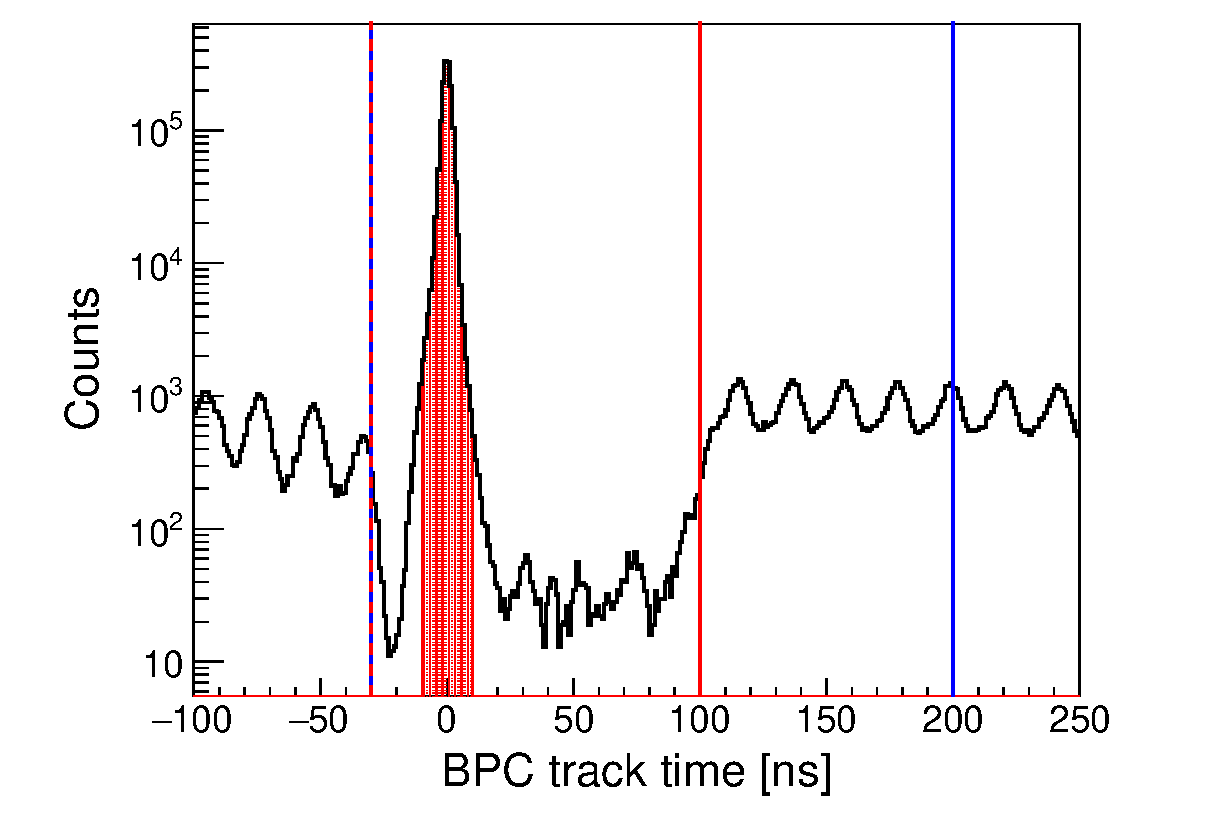
\includegraphics[width=4cm]{../pic/Run78/BL/BPC_time.eps}
    \end{minipage}
    \begin{minipage}{0.33\hsize}
      \includegraphics[width=4cm]{../pic/Run78/BL/nBPC.eps}
    \end{minipage}
    \begin{minipage}{0.33\hsize}
      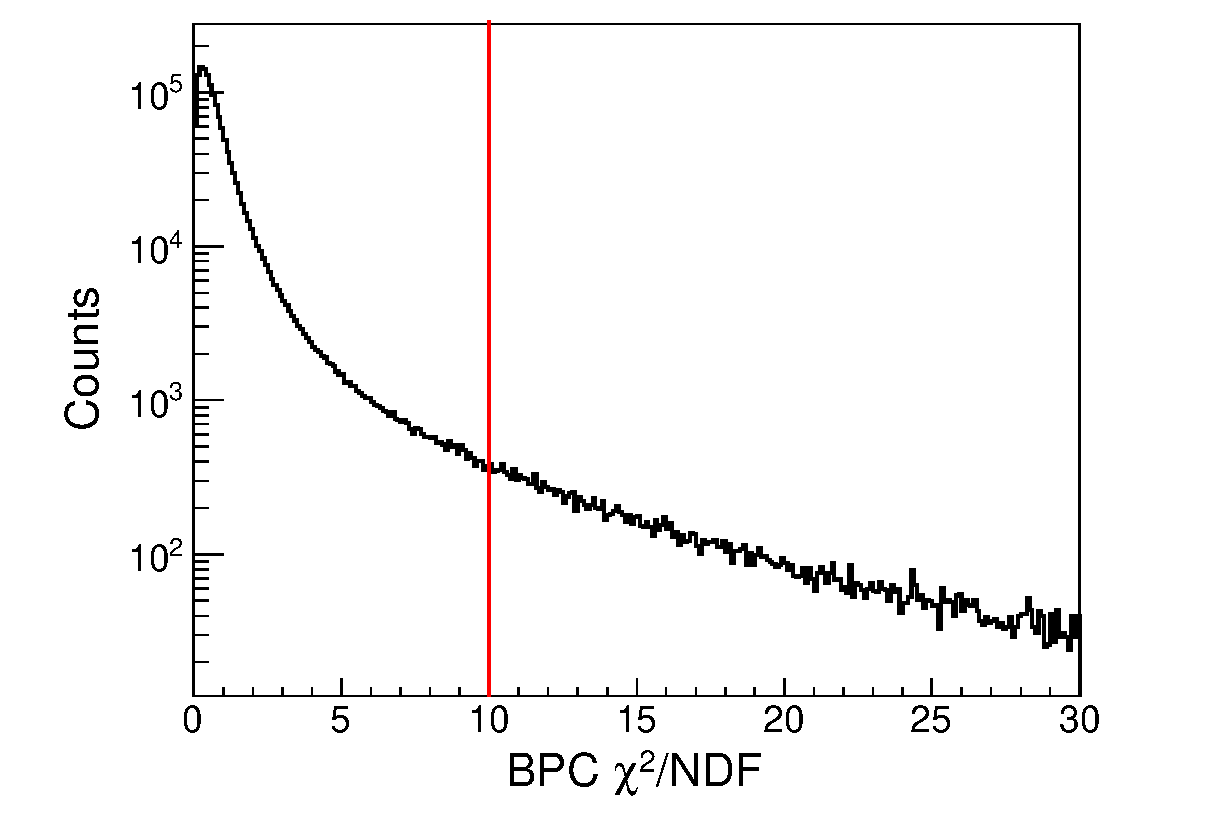
\includegraphics[width=4cm]{../pic/Run78/BL/BPC_chi2.eps}
    \end{minipage}
  \end{tabular}
  \caption{
    The left, the middle and the right figures show the number of tracks, track time and $\chi/NDF$, respectively.
    Color plots in the left figure indicate some time window.
    % Black, blue, red indicate all, $-30\sim200$[ns], $-30\sim100$[ns], respectively.
    The above, the middle and the down figures represent BLC1, BLC2 and BPC, respectively.
    The BPC was described after.
  }
  \label{fig:BLDC_selection}
\end{figure}


This subsection describes the selection in each chamber installed in the beamline.
Fig.\ref{fig:BLDC_selection} represents selection by chambers in the event identified as kaon by the TOF method.

They are planar drift chambers and the track is determined from the wire position and drift length.
The drift length of each pair of planes in that track corresponds to the length of the cell,
so the transit time of the particles can be determined by correcting the drift time corresponding to the length of the cell from the average time, which is shown in the left figures.
The gate accepted as events synchronised with the beam are set widely $-10 \sim 10$ns to leave more events.
Accepted events are indicated by red hatches.
Other events are accidental, these could be due to the influence of a device called transvese-RF with a period of 25ns for the SX, the structure of which is seen in the figure.
The $-30 \sim 100$ns reduction in events seen in BLC2 and BPC can be attributed to the gate of the T0 signal.

The center figure shows the number of tracks and the different colours represent the different timing gates according to track time.
Black, blue and red represent no gate, $-30 \sim 200$ns gate and $-30 \sim 100$ns gate respectively, with the range of gates indicate as vertical lines in the left figure.
In order to leave events that can be analysed, a $-30\sim 100$ns gate is set and requires that it is 1track within that gate.

The right diagram shows the reduced chi-square of the track synchronised with the beam, where $\chi^2/NDF<10$ is accepted as the correct track.
